\chapter{Machine Learning based Backtesting}

In the world of machine learning (ML), classification is about sorting things into categories. When applied to trading,
the ML Models predicts whether the price will go up or down based on today's as well as historical data from the past.
Using ML to predict trading outcomes requires a systematic approach.
This structured process is visualized as a pipeline, detailed in fig. \ref{fig:ml_pipeline}.

%trim=left bottom right top,
\section{Pipeline}


\begin{figure}[H]
\centering
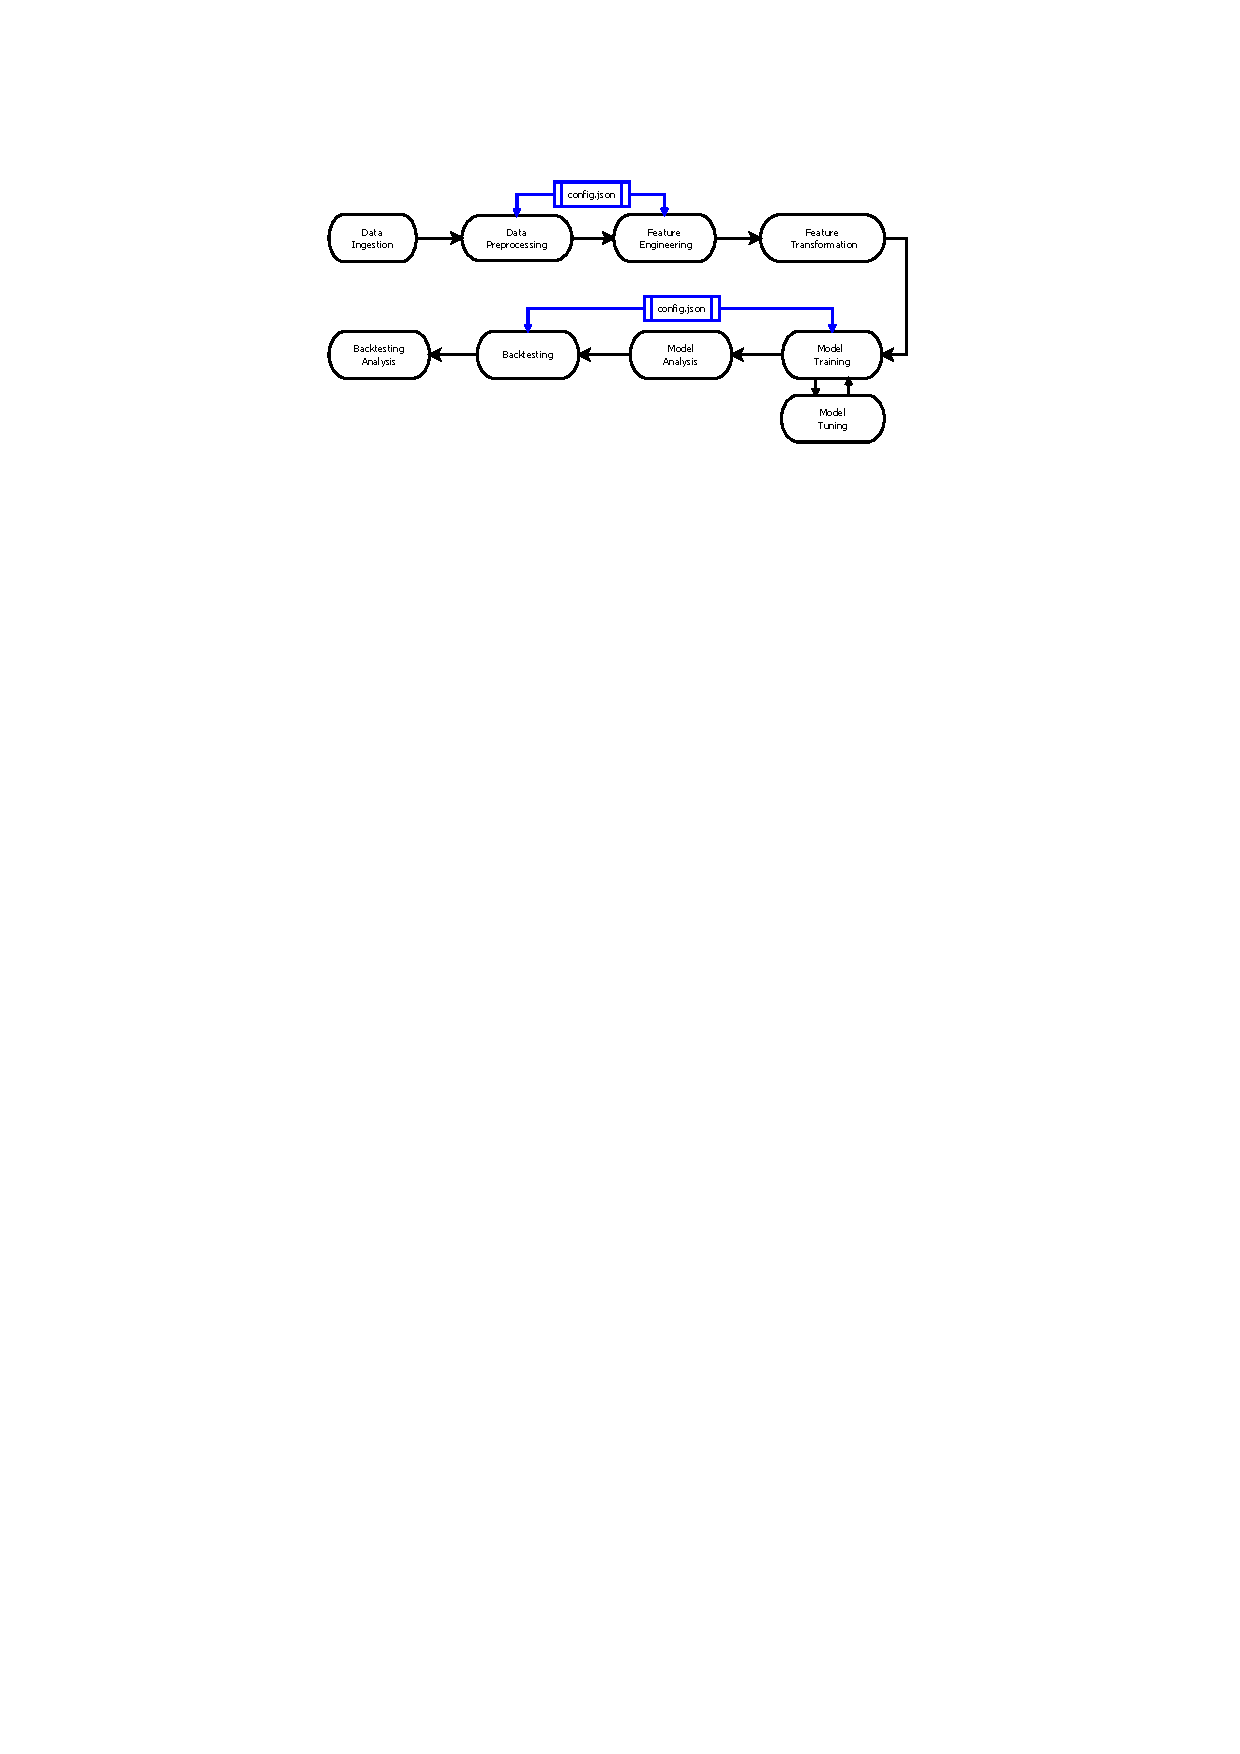
\includegraphics[trim=25mm 220mm 55mm 30mm, width=1.2\textwidth, clip]{./pdf/ml_pipeline.pdf}
\caption{Technical indicator based backtesting architecture.}
\label{fig:ml_pipeline}
\end{figure}

This pipeline initiates with raw historical data sourced from Binance and advances through a series of steps
leading to informed trading decisions. The process involves backtesting using the trained and optimized ML model on the historical data.
The pipeline steps can also be executed independently.
For instance, starting with data ingestion and preprocessing can be followed by feature engineering and data visualization to gain a deeper understanding of the dataset. The steps of the pipeline in  fig. \ref{fig:ml_pipeline}. are detailed in the subsequent subsections.

\subsection{Configuration}
The following JSON configuration in lst. \ref{lst:mlpipeline} is used to set up the machine learning pipeline.
The \texttt{dataset\_conf} element specifies details such as the cryptocurrency symbol (BTCUSDT in this case), the frequency of the time series data, and the start and end dates.
Additionally, it offers an option to set the date for splitting the dataset into training and test sets.
The configuration also includes options to set the desired model and the associated parameter space, facilitating fine-tuning via grid search.
Also the \texttt{target\_conf} element allows for the selection of the target for the classification model. There are several target variants to choose from, that are describe later.




\begin{lstlisting}[style=jsonstyle, caption={Machine Learning Pipeline Configuration}, label=lst:mlpipeline][h]
{
  "tc": 0.000750,
  "dataset_conf": {
     "symbol": "BTCUSDT",
     "freq": "1d",
     "start_date": "2018-01-01 00:00:00",
     "end_date": "2023-08-30 23:59:00",
     "split_date": "2022-12-31 23:59:00",
     "mode": "full",
     "target_conf": {
       "target": "Exceed_Avg_Returns"
    }
  },
  "model_name": "RandomForestClassifier",
  "model_type": "classification",
  "models_config": [
     {
       "model": "AdaBoostClassifier",
       "params": {
          "n_estimators": [10, 30, 100],
          "learning_rate": [0.01, 0.1, 1.0],
          "algorithm": ["SAMME", "SAMME.R"]
       }
     }
  ]
}
\end{lstlisting}



\subsection{Data Ingestion and Preprocessing}
The first step is to ingest the data needed for backtesting. This data can be obtained using the \texttt{dat\_retrieve.py} module,
as discussed in the previous chapter, or it can be loaded from the \texttt{historical\_data} folder located within the respective symbol's subfolder
If the data hasn't been previously downloaded, it can be found here. It's recommended to retrieve data with a one-minute time bar length,
as this can be efficiently downsampled later for larger intervals such as an hour or a day.
This is done in the data preprocessing phase, the ingested data is downsampled based on the bar length stipulated in the configuration. Furthermore, a validation check is run to ensure data integrity.

\begin{figure}[h]
\centering
\begin{adjustbox}{max width=1.15\textwidth,center}
    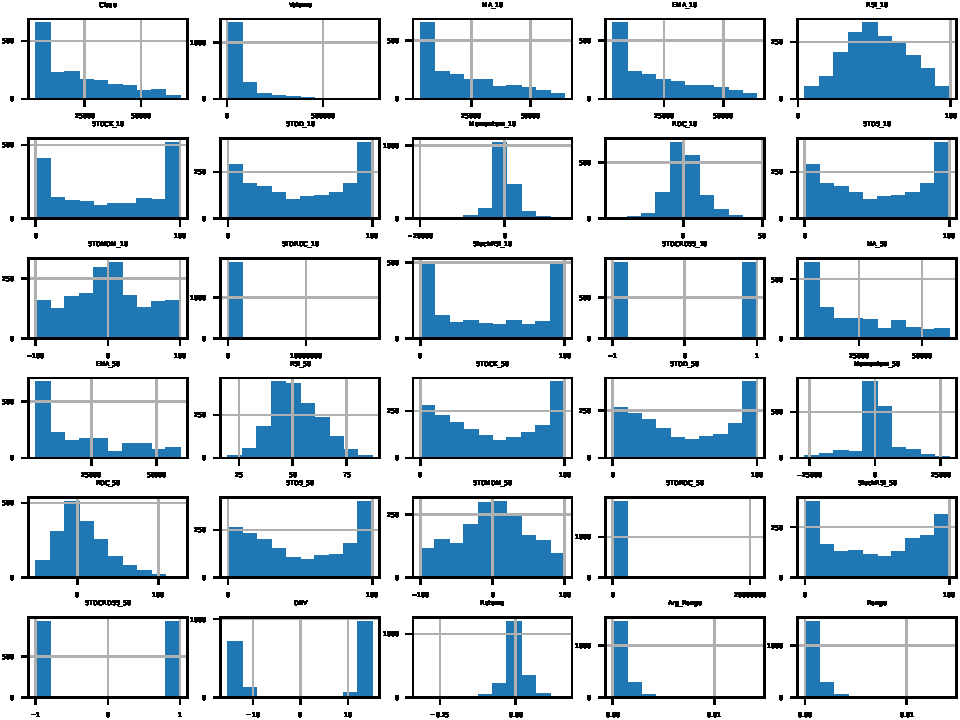
\includegraphics[scale=1.15]{./pdf/dataset_histogram.pdf}
\end{adjustbox}
\caption{Histogram of engineered features from the BTCUSDT historical data.}
\label{fig:dataset_histogram}
\end{figure}


%\vspace{20mm} % Put space between figure and subsection title
%\vspace{10mm} % Adjust the value to your liking
\FloatBarrier % This ensures that the figure is placed before continuing with the subsequent content
\subsection{Feature Engineering}
Feature engineering is a critical step in improving the model's predictive capability.
The goal is to identify features that could potentially influence the model's performance.
Technical indicators are utilized to create features that help models predict upcoming price movements based on historical market data.
The technical indicators used in the \texttt{ml\_feature\_engineer} module can be broadly categorized into momentum-based, trend-based, and volume-based.


\begin{itemize}
    \item \textbf{Momentum-based Indicators:} These are primarily concerned with the speed of price movements. Features like Rate of Change (ROC), Momentum, variations of the Stochastic Oscillator, and the Relative Strength Index (RSI) fall into this category.

    \item \textbf{Trend-based Indicators:} Aimed at identifying the movement direction over time, these include indicators such as the Moving Average (MA) and the Exponential Moving Average (EMA).

    \item \textbf{Volume-based Indicators:} Volume, in trading, refers to the number of shares or contracts traded in a security or market. The feature set for this category includes the On-Balance Volume (OBV).
\end{itemize}


Following this, a target is computed, which can also be specified in the configuration file. The available target variants include:
\begin{itemize}
    \item \textbf{Simple}: Predicts if the next day's price will go up or down based on today's closing price.
    \item \textbf{MA\_Relative}: Checks if today's closing price is above its short-term average and rising.
    \item \textbf{Momentum}: Examines if the stock's momentum is positive and increasing.
    \item \textbf{ROC}: Looks at if the rate of change (ROC) is positive and on the rise.
    \item \textbf{Consecutive\_Increases}: Predicts if returns will rise for the third consecutive time after a decline.
\end{itemize}


\begin{figure}[h]
\centering
\begin{adjustbox}{max width=1\textwidth,center}
    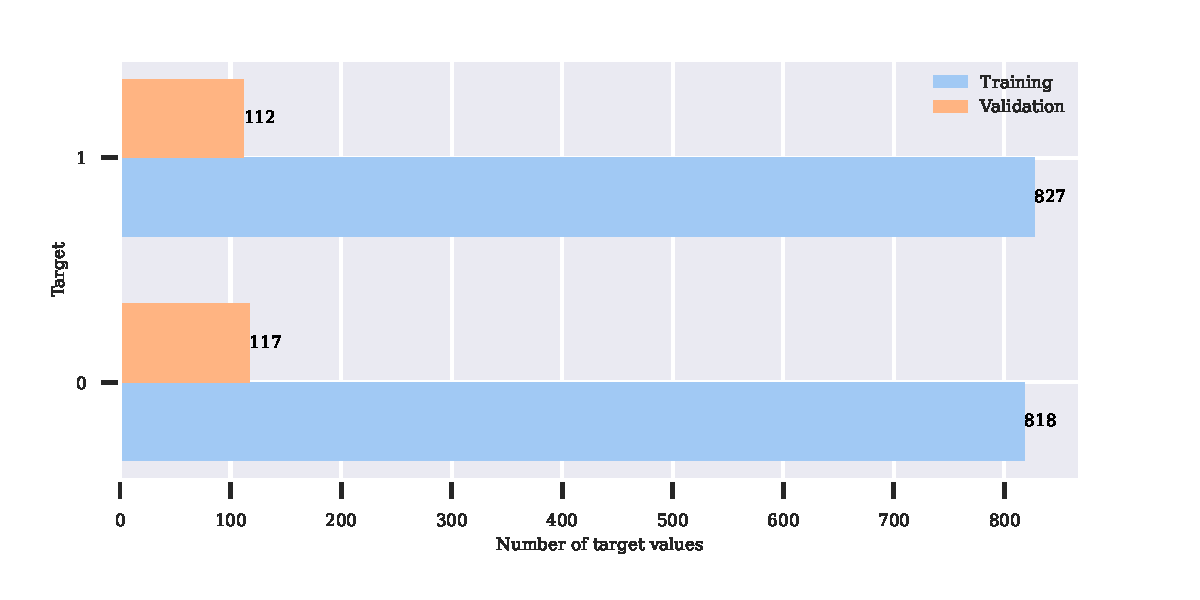
\includegraphics[scale=1]{./pdf/report/sig_distr.pdf}
\end{adjustbox}
    \caption{The distribution of target values in both the training (shown in green) and validation (shown in blue) datasets. Each horizontal bar represents a unique target value, with the length of the bar indicating the count of occurrences in the respective dataset. Absolute counts are annotated directly on the bars, facilitating a clearer understanding of the distribution. This visualization aids in discerning the balance or imbalance of target values across the two datasets.}
\label{fig:signal_distribution}
\end{figure}

 %Confusion matrix (left) presenting actual versus predicted values, alongside key performance metrics (right) indicating the model's accuracy, precision, recall, and F1 score.}
\subsection{Feature Transformation}

Once features have been engineered, it's essential to transform them to ensure they are adjusted to meet the requirements and sensitivities of machine learning models. Different models have varied preferences when it comes to the scale and distribution of input data. This transformation process uses several techniques such as Standardization and MinMaxScaling.

It's vital to apply the same transformations, like standardization parameters, to both the training and testing datasets or any new incoming data. This ensures consistent and accurate model predictions.

The entire transformation workflow, from data loading, preprocessing, to feature-related operations, is orchestrated by the \texttt{DataManager} and \texttt{FeatureEngineer} classes (fig. \ref{fig:dataManagerFeatureEngineer}).
After this step the \texttt{ml\_model\_evaluator} module can be used for data analysis. It provides tools for both data and model checks. The prepared data can be visualized in various ways, including target distributions, feature covariance matrices, and feature histograms.

\subsection{Data Visualization}
Let us look at the distribution of the predicted variable. The predicted variable is 1 more than 52\% of the time, meaning there are more buy
signals than sell signals. The predicted variable is relatively balanced, especially as
compared to the fraud dataset we saw in the first case study.


%trim=left bottom right top,
\begin{figure}[H]
\centering
\begin{adjustbox}{max width=1.2\textwidth,center}
    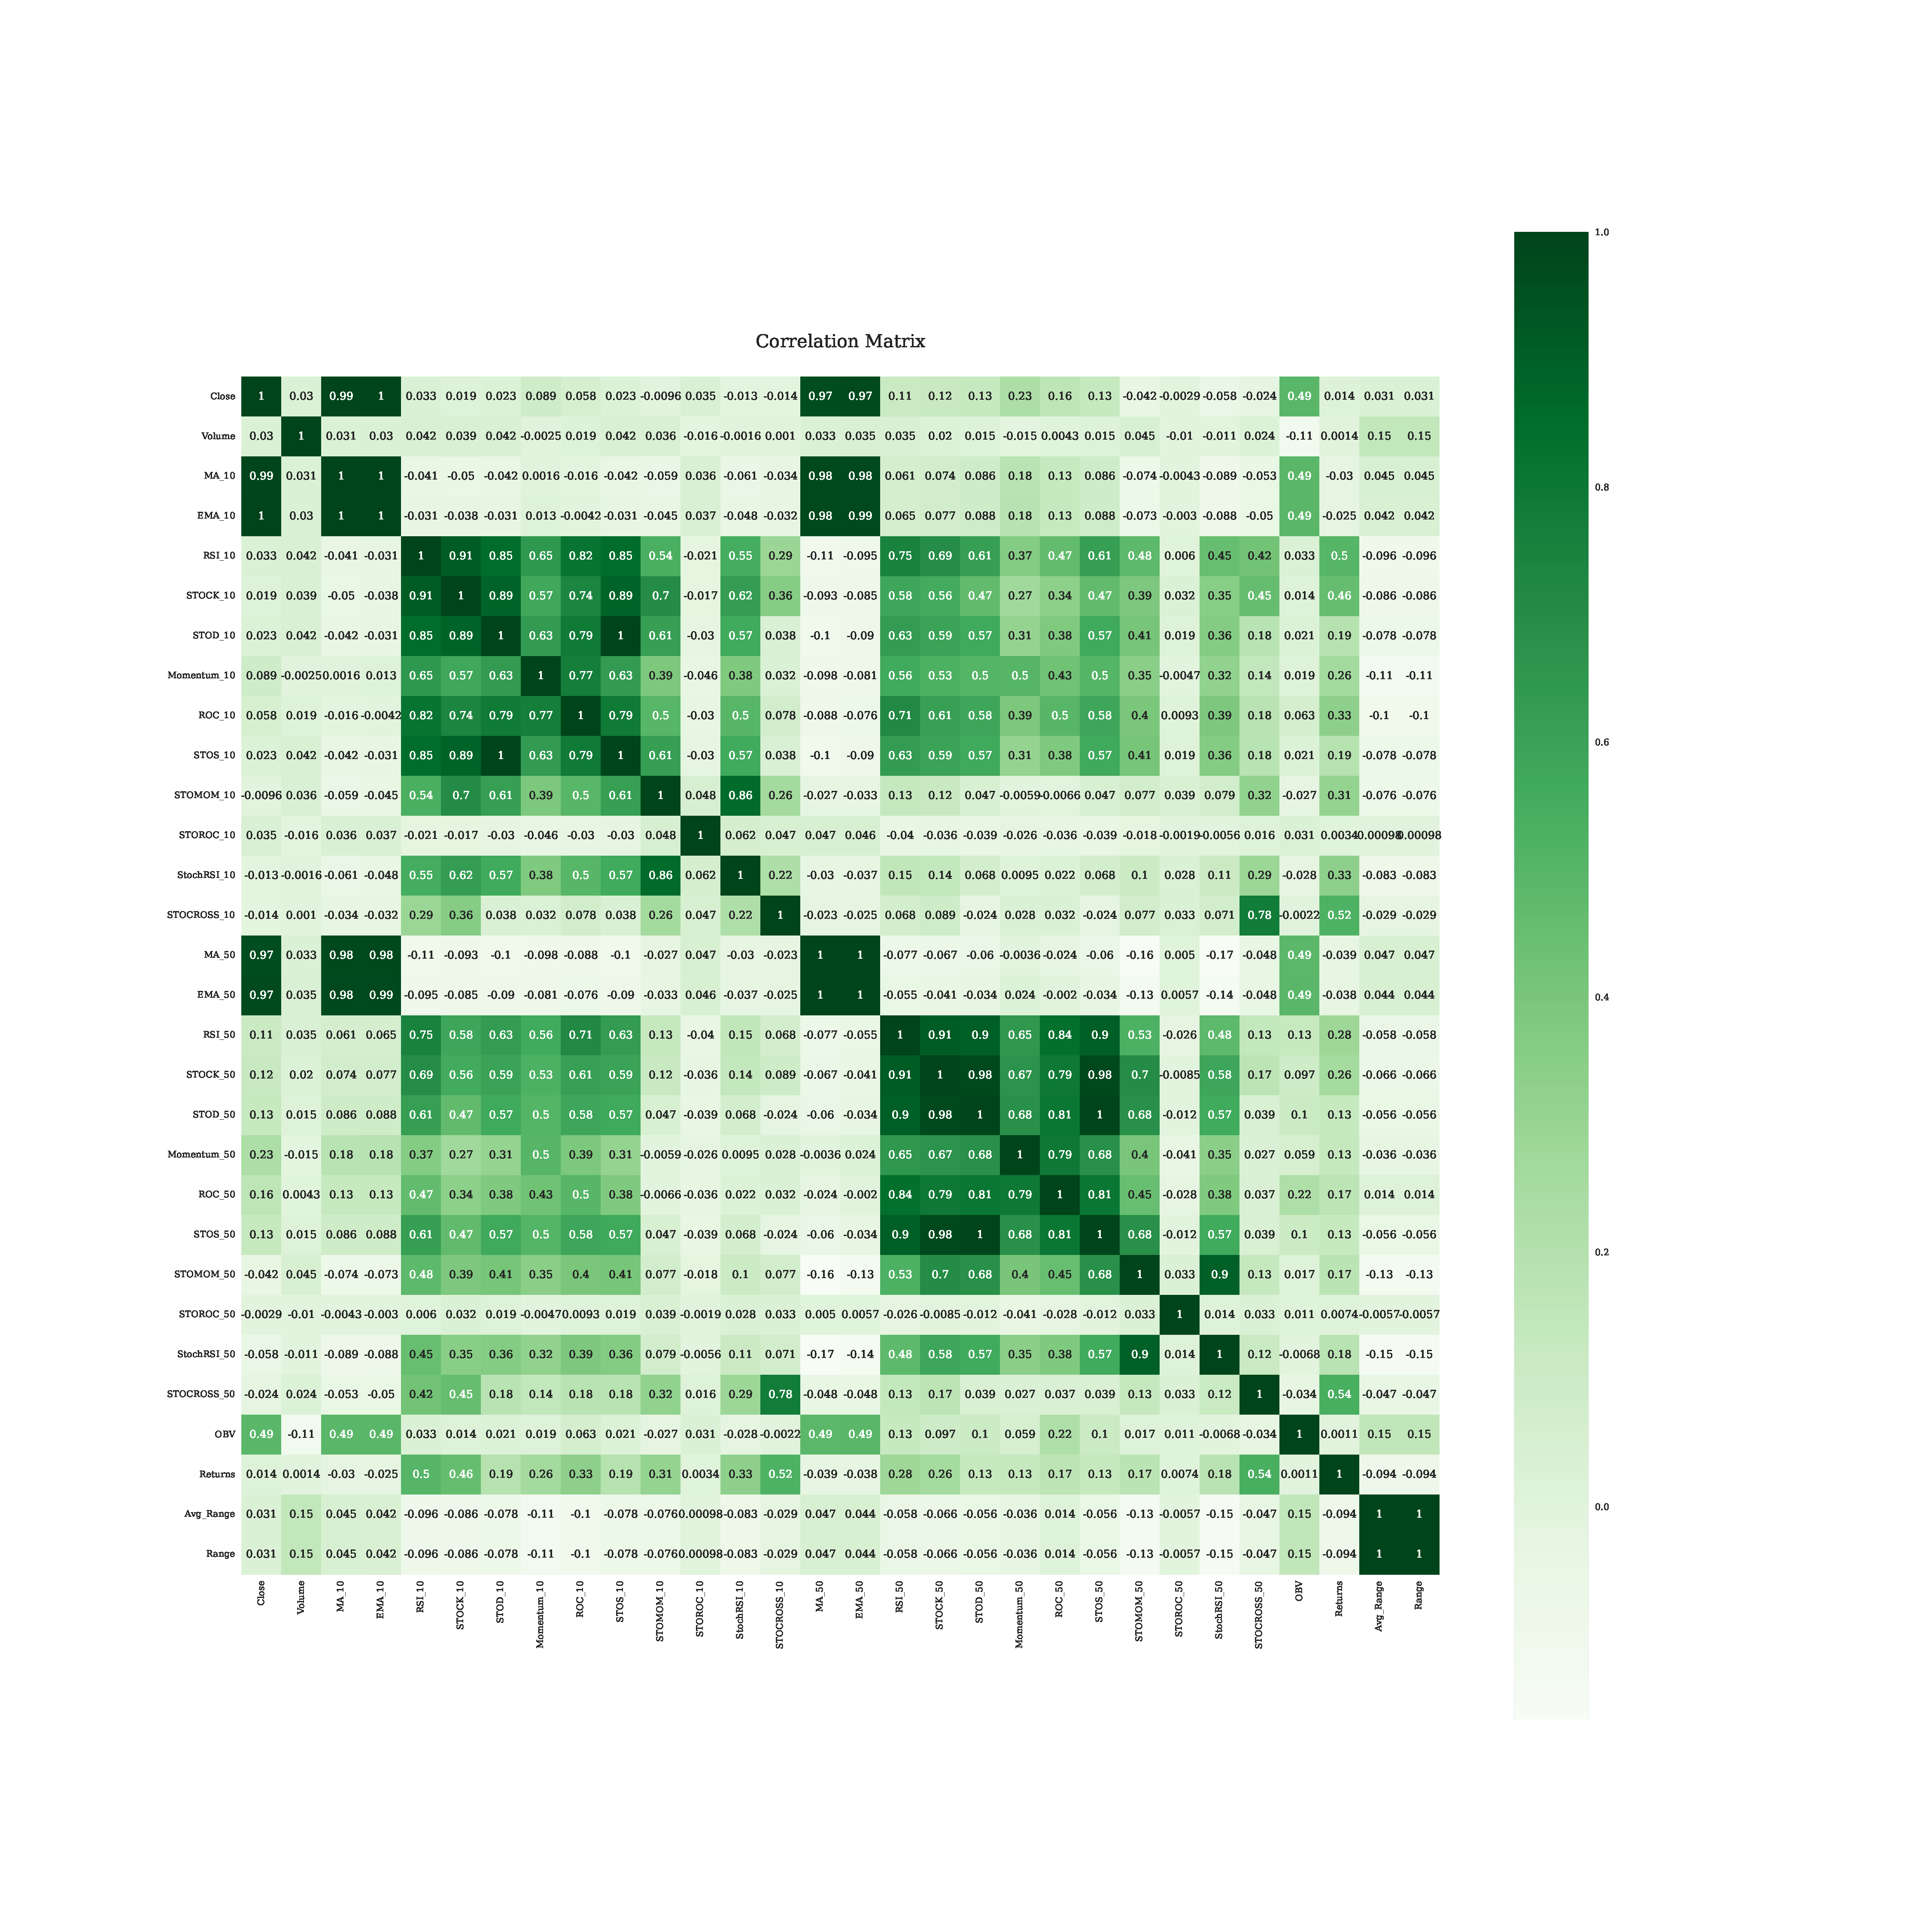
\includegraphics[scale=1.2, trim={30mm 70mm 50mm 110mm}, clip]{./pdf/correlation_matrix.pdf}
\end{adjustbox}
\caption{Correlation Coefficient between features variables.}
\label{fig:corr_coef}
\end{figure}


\subsection{Model Training and Optimization}
Model specifics, including the model type (e.g., LogisticRegressor) and its hyperparameter ranges, are detailed in the JSON configuration file. The optimization uses Grid Search combined with Cross-Validation, the details of which (e.g., number of folds) can also be adjusted in the configuration file (see fig. ~\ref{fig:modelConfig}).

\subsection{Model Evaluation using Classification Metrics}
After training the trading model's performance can be evaluated using several metrics. These metrics provide insights into the model's predictions and highlight potential areas for improvement.
The performance data for both the training and testing of the model are visualized in fig. \ref{fig:conf_matrix}.
For each phase (training and testing):

The left diagram presents the confusion matrix, which shows the number of correct and incorrect predictions made by the model.
The right diagram visualizes key performance metrics, specifically: accuracy, precision, recall, and F1 score. Each metric is also further described in  more detail below.
\begin{figure}[H]
    \centering

    \begin{subfigure}[b]{\textwidth}
        \begin{adjustbox}{max width=0.8\textwidth,center}
            \includegraphics[scale=0.8]{./pdf/report/report\_train.pdf}
        \end{adjustbox}
        \caption{Model Performance Metrics based on Training Data.}
        \label{fig:train_perf}
    \end{subfigure}

    \bigskip % Adds some vertical space between the two subfigures

    \begin{subfigure}[b]{\textwidth}
        \begin{adjustbox}{max width=0.8\textwidth,center}
            \includegraphics[scale=0.8]{./pdf/report/report\_test.pdf}
        \end{adjustbox}
        \caption{Model Performance Metrics based on Testing Data.}
        \label{fig:test_perf}
    \end{subfigure}

    \caption{Visualization of the Classification Report.}
    \label{fig:conf_matrix}
\end{figure}

\begin{itemize}
	\item \textbf{True Positive:} Represents the number of times the model correctly predicted an upward trend and the price actually went up.

	\item \textbf{True Negative:} Represents the number of times the model correctly predicted a downward trend and the price actually went down.

	\item \textbf{False Positive:} Represents the number of times the model incorrectly predicted an upward trend and the price went down or stayed the same. This type of error could result in a missed shorting opportunity or a loss if one decided to buy in Long Only strategies.

	\item \textbf{False Negative:} Represents the number of times the model incorrectly predicted the downward trend and the price went up or stayed the same. This type of error could result in missed profit opportunities from not buying.

	\item \textbf{Recall:} The ratio of the number of correct positive predictions (TP) to the total actual positives (TP + FN). In mathematical terms, Recall $= \frac{TP}{TP + FN}$. In trading, it indicates how well the model identifies actual upward movements. A high recall means the model captures most of the upward trends, but this can also be achieved at the expense of more false positives.

	\item \textbf{Precision:} The ratio of correct positive predictions (TP) to the total predicted positives (TP + FP). In mathematical terms, Precision $= \frac{TP}{TP + FP}$. Shows how many of the predicted upward trends by the model were actually correct. High precision means that when the model predicts an upward trend, it's likely correct. But a higher precision might come at the expense of missing some actual upward trends (lower recall).

	\item \textbf{Accuracy:} The ratio of correct predictions (both TP and TN) to the total number of predictions (TP + TN + FP + FN). In mathematical terms, Accuracy $= \frac{TP + TN}{TP + TN + FP + FN}$. In trading, it gives an overall measure of how often the model is correct, regardless of whether it's predicting upward or downward movement.

	\item \textbf{F1 Score:} The harmonic mean of precision and recall, providing a balance between the two. It is given by the formula: F1 $= 2 \times \frac{\text{Precision} \times \text{Recall}}{\text{Precision} + \text{Recall}}$. It's especially useful when the class distribution is imbalanced. In trading, a high F1 score suggests the model has a balanced performance in terms of identifying upward trends and avoiding false alarms.
\end{itemize}


\begin{figure}
\centering
\begin{adjustbox}{max width=1.2\textwidth,center}
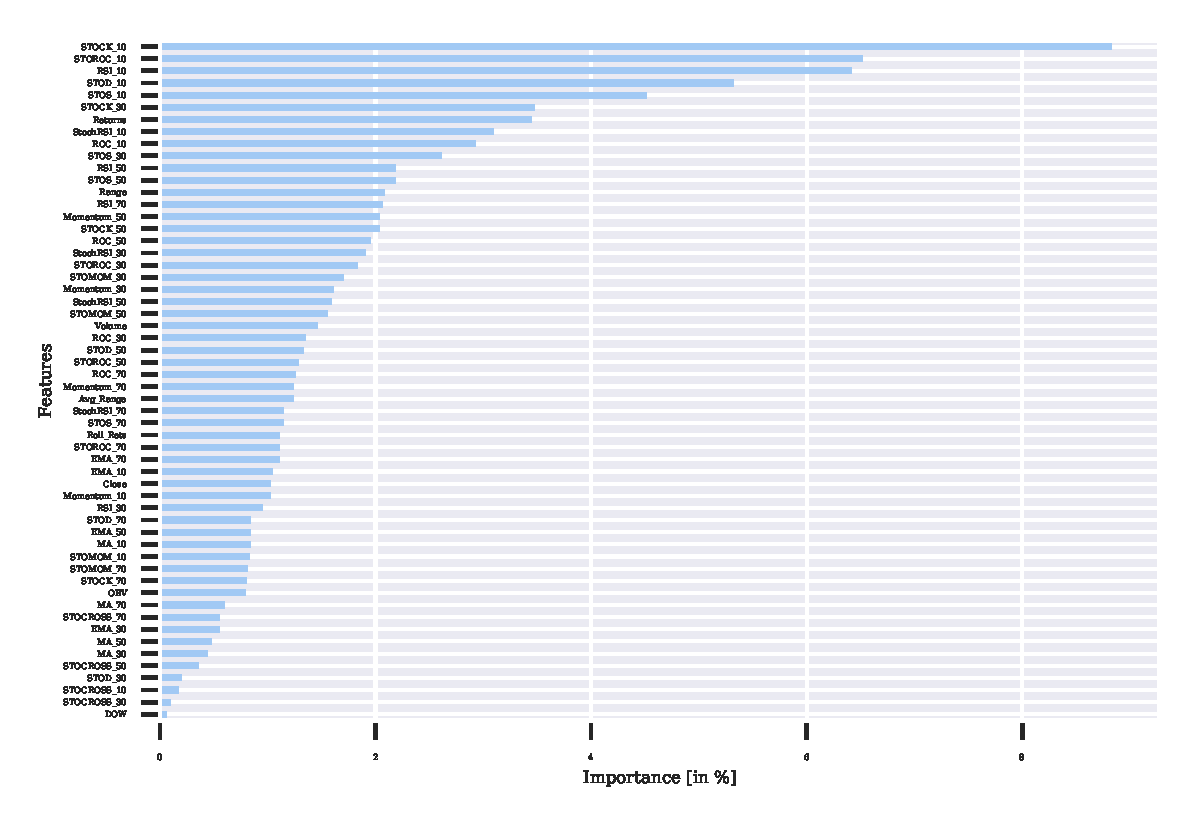
\includegraphics[scale=1.2]{./pdf/report/feature_importance.pdf}
\end{adjustbox}
\caption{Feature Significance in Model Prediction}
\label{fig:feature_importance}
\end{figure}


\subsection{Backtesting}

In this additional step, we perform a backtest on the model
we’ve developed. We create a column for strategy returns by multiplying the daily
returns by the position that was held at the close of business the previous day and
compare it against the actual returns.

Backtesting is done in a separate step because it has its unique methods and processes. The trained and adjusted model is tested to see the returns, showing how it might have worked in real-life situations.
\subsection{Backtest Analysis}
The last step in the evaluation of backtesting results. Performance metrics in this analysis include strategy returns, comparison to a benchmark like the buy-and-hold strategy, and the usage of other advanced metrics such as Calmar and Sortino ratios.

Looking at the backtesting results, we do not deviate significantly from the actual
market return. Indeed, the achieved momentum trading strategy made us better at
predicting the price direction to buy or sell in order to make profits. However, as our
accuracy is not 100% (but more than 96%), we made relatively few losses compared
to the actual returns.


\begin{figure}
\centering
\begin{adjustbox}{max width=1.3\textwidth,center}
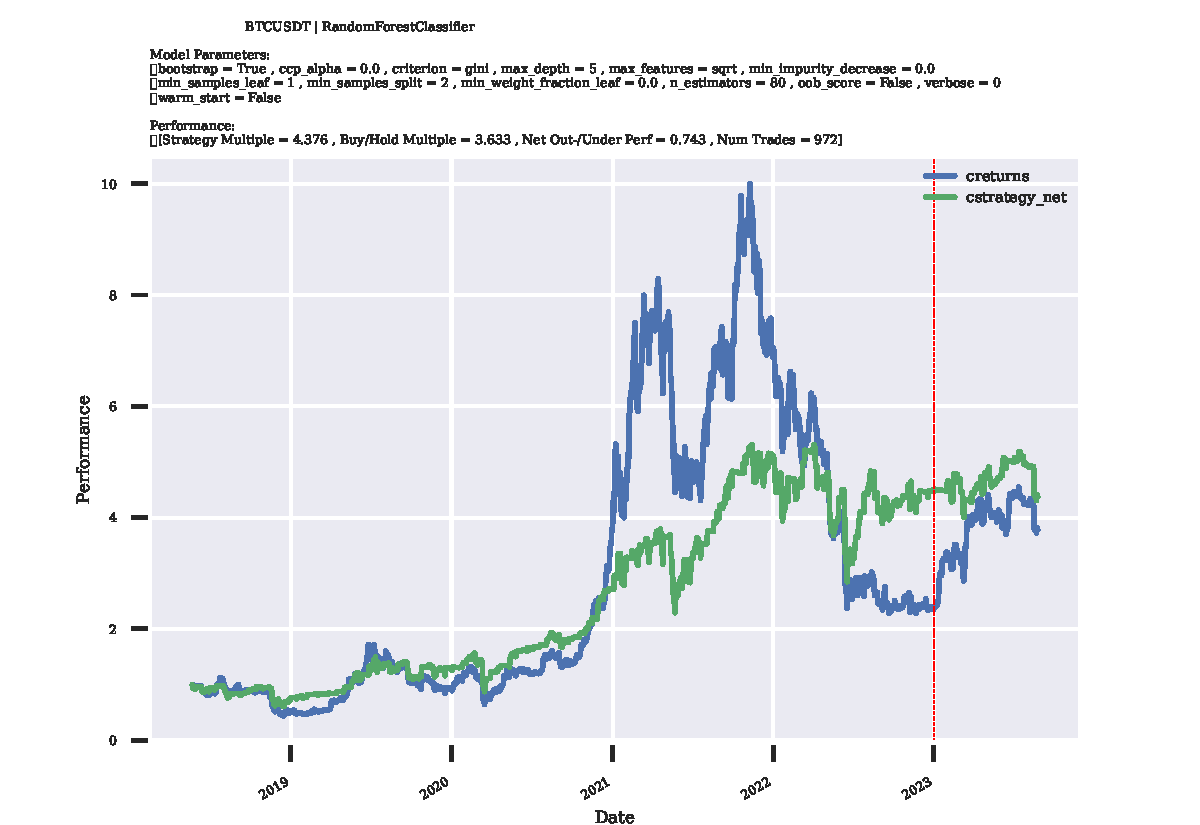
\includegraphics[scale=1.3]{./pdf/report/backtest_res.pdf}
\end{adjustbox}
\caption{Feature Significance in Model Prediction}
\label{fig:backtest_res}
\end{figure}




\begin{figure}
\centering
\includegraphics[width=0.9\textwidth]{./pdf/report/explained\_variance.pdf}
\caption{Explained Variance of Features after Performing Feature Reduction.}
\label{fig:explained_variance}
\end{figure}
